
%%%%%%%%%%%%%%%%%%%%%%% file typeinst.tex %%%%%%%%%%%%%%%%%%%%%%%%%
%
% This is the LaTeX source for the instructions to authors using
% the LaTeX document class 'llncs.cls' for contributions to
% the Lecture Notes in Computer Sciences series.
% http://www.springer.com/lncs       Springer Heidelberg 2006/05/04
%
% It may be used as a template for your own input - copy it
% to a new file with a new name and use it as the basis
% for your article.
%
% NB: the document class 'llncs' has its own and detailed documentation, see
% ftp://ftp.springer.de/data/pubftp/pub/tex/latex/llncs/latex2e/llncsdoc.pdf
%
%%%%%%%%%%%%%%%%%%%%%%%%%%%%%%%%%%%%%%%%%%%%%%%%%%%%%%%%%%%%%%%%


\documentclass[runningheads,a4paper]{llncs}

\usepackage{amssymb}
\usepackage{wrapfig}
\setcounter{tocdepth}{3}
\usepackage{graphicx}
\usepackage{amsmath}
\usepackage{subfigure}
\usepackage{verbatim} 
\usepackage[hyphens]{url}
\usepackage{fixltx2e}
\usepackage{textcomp}
\usepackage{listings}
\lstset{
        basicstyle=\ttfamily\scriptsize,
        upquote=true,
        showspaces=false,
        showstringspaces=false,
        showtabs=false,
        tabsize=2,
        frame=none,
        breaklines,
        numbers=none,
        framexleftmargin=2mm,
        xleftmargin=2mm,
}

\usepackage{url}
\newcommand{\keywords}[1]{\par\addvspace\baselineskip
\noindent\keywordname\enspace\ignorespaces#1}

%% Define a new 'smallurl' style for the package that will use a smaller font.
\makeatletter
\def\url@smallurlstyle{%
  \@ifundefined{selectfont}{\def\UrlFont{\sf}}{\def\UrlFont{\scriptsize\ttfamily}}}
\makeatother
%% Now actually use the newly defined style.
\urlstyle{smallurl}
\newcommand{\nofootnote}[1]{~#1}

\begin{document}

\mainmatter  % start of an individual contribution

% first the title is needed
\title{A Tweet Consumers' Look At Twitter Through Linked Data Goggles Via Google Analytics}

% a short form should be given in case it is too long for the running head
\titlerunning{A Tweet Consumers' Look At Twitter}
\authorrunning{A Tweet Consumers' Look At Twitter}

% the name(s) of the author(s) follow(s) next
%
% NB: Chinese authors should write their first names(s) in front of
% their surnames. This ensures that the names appear correctly in
% the running heads and the author index.
%
\author{Thomas Steiner\inst{1} \and Arnaud Brousseau\inst{1,2}\thanks{The author is a graduate student at EURECOM, Sophia Antipolis (France), and currently works as an intern at Google Germany GmbH.} \and Rapha\"{e}l Troncy\inst{2}}

\institute{
  Google Germany GmbH, ABC-Str. 19, 20354 Hamburg, Germany\\ \email{\{tomac,arnaudb\}@google.com} \and
  EURECOM, Sophia Antipolis, France\\ \email{raphael.troncy@eurecom.fr}
}

%
% NB: a more complex sample for affiliations and the mapping to the
% corresponding authors can be found in the file "llncs.dem"
% (search for the string "\mainmatter" where a contribution starts).
% "llncs.dem" accompanies the document class "llncs.cls".
%


\maketitle

\begin{abstract}
The Twitter Trends feature allows for a global or local view on ``what's happening in my world right now" from a tweet producers' point of view. In this paper, we show the possibility to complete the functionality provided by Twitter Trends via having a closer look at the other side: the tweet consumers' -- i.e., readers' -- point of view. While Twitter Trends works by analyzing the frequency of terms and their velocity of appearance in tweets being written, our approach is based on the popularity of extracted named entities (in the sense of Linked Data) in tweets being read. Our experimentation architecture uses a client-side browser extension to harvest and dissect tweets from users' timelines, search result pages, or profile pages, i.e., tweets supposed to be read. Named entities are extracted via several third-party Natural Language Processing (NLP) Web services in parallel, and are then reported to Google Analytics, which is used to store, analyze, and compute trends by pivoting the reported named entities by Google Analytics data, e.g., users' geographic locations.
\end{abstract}

\section{Introduction}\label{sec:introduction}
The Twitter Trends feature was introduced by Twitter in September 2008 with the objective to reflect ``what's happening in my world right now" in the beginning only globally\footnote{\url{http://blog.twitter.com/2008/09/twitter-trends-tip.html}}, but since January 2010 also locally\footnote{\url{http://blog.twitter.com/2010/01/now-trending-local-trends.html}}. To compute trends, Twitter uses an algorithm which analyzes the words and hashtags in tweets. Although the concrete implementation details are kept secret, it is known\footnote{\url{http://blog.twitter.com/2010/12/to-trend-or-not-to-trend.html}} that the algorithm considers three main characteristics of terms/hashtags to determine whether they are part of a ``trend":

\begin{itemize}
\item The \textbf{quantity}, i.e, the absolute number of appearances of a given term/hashtag among all users' tweets.
\item The \textbf{velocity}, i.e, the frequency of appearance of that term/hashtag. The higher the frequency, the more popular the term/hashtag.
\item The \textbf{newness}, e.g, the (at the time of writing brand new) hashtag \texttt{\#ipad2} would be given priority over an old and generic tag like \texttt{\#awesome} to be featured as ``trend".
\end{itemize}

\begin{comment}
\begin{figure}[ht!]
  \centering
    \includegraphics[width=0.17\linewidth]{twitter-trends.png}
  \caption{Screenshot of Twitter Trends as of Friday, March 4, 2011, 4pm CET.}
  \label{fig:trends}
\end{figure}
\end{comment}

Twitter Trends analysis is a fascinating field to many, with both an academic or an industry (or even social media hobbyist) background (e.g., \cite{Kannan:Trendtracker} by Kannan et al. gives a good overview of Twitter Trends analysis and visualization efforts). What all these approaches have in common is that they focus on the tweet producers' point of view: either they are based on the output from the Twitter Trends API\footnote{\url{http://dev.twitter.com/doc/get/trends/}} (i.e., use Twitter's pre-calculated trends data), or use the Twitter Streaming API\footnote{\url{http://dev.twitter.com/pages/streaming_api}} (i.e., calculate trends data on their own). What to the best of our knowledge has been missing so far is the tweet consumers' point of view. If many Twitter users tweet about a topic, this does not necessarily mean that tweet consumers also read these tweets. Currently the closest practical approximation to estimate whether a tweet (on Twitter.com, not in third-party applications) has been read is to check whether it has ever appeared on someone's timeline, search result page, or profile page (the tweet producer having followers alone is not a sufficient condition). A different approach would be to only count tweets as read if potentially contained URLs have been clicked. This leaves out many potentially read tweets that either do not contain URLs, or only unclicked URLs.

In this paper, we suggest a solution for enabling tweet tracking combined with named entity extraction (NEE) for the Twitter.com page. This solution allows to combine data from classic Web analysis (such as user location) with our interpretation of Twitter trends, which is based on named entities. Others\footnote{E.g., \url{http://trendsmap.com/}} have created visualizations of user location combined with trends, however, user location so far has been an approximation of what Twitter users expose on their Twitter profile pages, which is not necessarily the same as their current physical location, but oftentimes their permanent hometown. 

The remainder of the paper is structured as follows: Section~\ref{sec:reqtec} introduces the two background technologies Google Chrome extensions and Google Analytics that are required for our experiment. Section~\ref{sec:twitterswarm} introduces our Twitter Swarm NLP Google Chrome extension. Section~\ref{sec:evaluation} contains an evaluation of our experimentation results so far. Section~\ref{sec:relatedwork} gives an overview on related work. Section~\ref{sec:conclusion} finalizes the paper with an outlook on future work, and gives a conclusion.

\section{Required Technologies}\label{sec:reqtec}
We begin with an overview of the used technologies for this experiment, namely we introduce Google Chrome extensions for the Google Chrome browser, and give a brief summary of the Web analysis solution Google Analytics.

\subsection{Google Chrome Extensions}
Google Chrome extensions\footnote{\url{http://code.google.com/chrome/extensions/index.html}} are small software programs that can be installed to enrich the browsing experience with the Google Chrome browser. They are written using a combination of standard Web technologies, such as HTML, JavaScript, and CSS. Chrome extensions get usually (but not necessarily) distributed through the Chrome Web Store\footnote{\url{https://chrome.google.com/webstore/}}. There are several types of extensions, for this paper we focus on extensions based on so-called content scripts. Content scripts are JavaScript programs that run in the context of Web pages via dynamic code injection, similar to the Firefox Greasemonkey extension\footnote{\url{http://www.greasespot.net/}}. By using the standard Document Object Model (DOM), they can read or modify details of the Web pages a user visits. An example of such modification is, e.g., removing background images for better legibility. Content scripts can run on any website, or be limited to just certain websites. This can be controlled by the extension developer with a so-called manifest file in JSON format. When a user installs an extension, the access rights of the extension are displayed and must be acknowledged by the user.

\subsection{Google Analytics}
Google Analytics\footnote{\url{http://www.google.com/analytics/}} is Google's Web analysis solution allowing for detailed statistics about the visitors of a website. The software is implemented by adding an invisible snippet of JavaScript code on the to-be-tracked pages of a website. This code collects visitor data through requests for a specific 1~x~1 pixel image on Google's servers, during which the page and user data is reported in the query part of the image's URL. In addition to that, the snippet sets a first party cookie on visitors' computers in order to store anonymous information such as the timestamp of the current visit, whether the visitor is a new or returning visitor, and the referrer of the website that the visitor came from. Part of the shared visitor information is the IP address, which allows for IP-based geolocation.
 
\section{Twitter Swarm NLP Extension}\label{sec:twitterswarm}
We have developed a Google Chrome extension called Twitter Swarm NLP\footnote{\url{https://chrome.google.com/webstore/detail/dpbphenfafkflfmdlanimlemacankjol}} which with we inject JavaScript code via a content script into the Twitter.com homepage. By installing this extension, users explicitly opt-in to their data as a Twitter.com visitor being tracked by Google Analytics. The extension first checks if the user is logged in to Twitter.com, and if so, retrieves the tweets of the current user's timeline (\url{http://twitter.com/#}), or search result page (e.g., \url{http://twitter.com/#!/search/%23semweb}), or profile page (e.g., \url{http://twitter.com/#!/timberners_lee}) on a one-by-one basis, and performs Named Entity Extraction (NEE) via Natural Language Processing (NLP) using a remote NLP Web service (see Section~\ref{sec:webservice}) on each of the tweets. The extracted entities are then displayed on the righthand-column of the Twitter.com homepage (see Figure~\ref{fig:danbri}), and sent to Google Analytics for further processing (see Section~\ref{sec:evaluation}).

\begin{figure}[ht!]
  \centering
  \includegraphics[width=0.56\linewidth]{danbri.png}
  \caption{Screenshot of the original tweet above, and the thereof extracted entities below.}
  \label{fig:danbri}
\end{figure}

\begin{comment}
\begin{figure}[ht!]
  \centering
  \includegraphics[width=0.8\linewidth]{analytics.png}
  \caption{Named entities pivoted by countries/territories. The named entity represented by the URL \texttt{http://dbpedia.org/resource/Libya} appeared in nine tweets read by users located in Finland (red borders in the screenshot).}
  \label{fig:analytics}
\end{figure}
\end{comment}

\subsection{Twitter Swarm NLP Web Service}\label{sec:webservice}
For our extension, we have created a wrapper NLP Web service that merges results from existing third-party NLP Web services, namely from OpenCalais\footnote{\url{http://www.opencalais.com/}}, Zemanta\footnote{\url{http://www.zemanta.com/}}, AlchemyAPI\footnote{\url{http://www.alchemyapi.com/}}, and DBpedia\cite{Bizer:DBpedia} Spotlight\footnote{\url{http://dbpedia.org/spotlight}}. All NLP Web services return named entities together with their types and potential subtypes, names, relevance, and URIs that link into the Linked Open Data (LOD) cloud\footnote{\url{http://lod-cloud.net/}}. The problem is that each service has implemented its own type system (e.g., the type ``city" is represented by \url{http://dbpedia.org/ontology/City} in DBpedia vs. \url{http://rdf.freebase.com/ns/location.citytown} in Freebase). Providing mappings for all of them would be a rather time-consuming task. However, as all services offer links into the LOD cloud, the type information can be pulled from there if need be, in a true Linked Data manner. In order to clarify what data our wrapper service provides, the merged results for the sample query ``Google Translate'' are depicted below. For the sake of clarity, we just show a shortened form (the complete result can be seen at the URL \url{http://tomayac.no.de/entity-extraction/combined/Google%20Translate}).

\begin{lstlisting}
[
  {
    "name": "Google Translate",
    "relevance": 0.7128319999999999,
    "uris": [
      {
        "uri": "http://dbpedia.org/resource/Google_Translate",
        "source": "alchemyapi"
      }
    ],
    "source": "alchemyapi"
  }
]
\end{lstlisting}

\subsection{Technical Implementation Of the Extension}\label{sec:techimp}
Twitter.com is an Ajax-dependent website, which makes use of so-called hashbang URIs\footnote{See \url{http://www.jenitennison.com/blog/node/154} for a Twitter hashbang URI analysis.}. When the page Twitter.com gets loaded, the static parts of the page can be cached, while the dynamic parts -- controlled by the content of the hashbang URI -- get pulled in via JavaScript. Currently the extension is implemented in a way to run once upon page load, however, not upon Ajax refresh events on the page.

We overload Google Analytics event tracking\footnote{\url{http://code.google.com/apis/analytics/docs/tracking/eventTrackerGuide.html}} for the purpose of tracking named entities. We interpret a Google Analytics event as the occurrence of a named entity in a tweet never seen before. In its original sense, event tracking is meant to track on-page events, like, e.g., playing or stopping an embedded video on a page. The anatomy of an event is as follows: an event is defined by its \texttt{category} (req.), \texttt{action} (req.), \texttt{label} (opt.), and \texttt{value} (opt.). In our concrete case, the \texttt{category} is always ``Entities", the \texttt{action} is any of the particular named entity's URIs (as they all represent the same thing, we simply choose the first URI of the list). The \texttt{label} is the particular entity's name and the sources of that named entity in parenthesis (as outlined in Section~\ref{sec:webservice}), and finally for the \texttt{value} we pass the timestamp of the moment where the entity extraction happened (which is closest to when we assume the tweet was read). A concrete call to log an occurrence of a named entity as injected onto Twitter.com by the content script looks like this (the \texttt{\_gaq} array is the Google Analytics queue for asynchronous tracking):

\begin{lstlisting}
_gaq.push(['twitter_swarm_nlp._trackEvent',
    'Entities',
    'http://dbpedia.org/resource/JSON',
    'json (zemanta,opencalais)',
    1299776578]);
\end{lstlisting}

Currently the extension displays all extracted named entities grouped by originating tweets and roughly in the tweet order at the righthand-column (see Figure~\ref{fig:danbri} for a screenshot). In order not to flood the Twitter Swarm NLP Web service (and in turn the underlying third-party NLP Web services), the NLP requests get sent in intervals of one second. Dependent on the response time for each particular request, the extracted named entities get added to the righthand-column. Each named entity is displayed with its label, one representing URI (out of potentially several URIs), and the sources.

\subsection{Avoiding Duplicate Tracking}
Each tweet gets sent one-by-one to the Twitter Swarm NLP Web service, as described in Section~\ref{sec:techimp}. While the extracted named entities of all tweets always get displayed to the user (as shown in Figure \ref{fig:danbri}), only named entities from tweets never seen before get sent to Google Analytics. This is to ensure that duplicate data from the same user does not falsify the overall statistics. It is to be noted that we do allow the same tweet to be tracked more than once (because one tweet can be read by more than one user), however, we want to exclude the case that the same tweet gets tracked more than once from the same user (we assume each tweet gets read at most one time). Twitter has introduced a new system to generate unique tweet IDs called snowflake\footnote{\url{https://github.com/twitter/snowflake#readme}}, which guarantees k-sorted IDs\footnote{See \url{http://portal.acm.org/citation.cfm?id=70413.70419}} with at least a 1s bound. This allows us to store the ID of the latest tweet in the extension's local storage, and check whether the current tweet's ID is greater (i.e., the tweet is younger than the previous latest tweet and has thus not been seen before), and only if so, send its named entities to Analytics. While this strict limitation to only consider new tweets leaves out many old tweets from being tracked in Analytics, it is the only alternative to storing the ID of each and all tweets in local storage to assure duplication-free tracking.

\section{Evaluation And Discussion}\label{sec:evaluation}
In this section we first provide some raw statistics followed by an evaluation of our experiments, and discuss the approach and its criticisms in the second part. If not noted differently, all statistics are for February 24 to March 11, 2011.

\subsection{Raw Statistics}
The extension was live since February 24, 2011. It was announced via Twitter\footnote{\url{http://twitter.com/#!/tomayac/status/40806491510276096}} on that day, and according to Bit.ly statistics\footnote{\url{http://bit.ly/eBsjQu+}} generated \textit{102 clicks} till March 11 (see Figure~\ref{fig:edge-a}). If we compare these click statistics of the announcement link with the pageview statistics according to Google Analytics (see Figure~\ref{fig:edge-b}), we can see interesting patterns. In the Bit.ly statistics there are two spikes on February 24 and 26, in the prior case originating from initial clicks on the link in the announcement tweet plus same-day retweets, and in the latter case originating from delayed retweets from people who found the extension interesting after testing it, together with a second announcement tweet on February 26. The top usage spike according to Analytics is around February 28 to March 2, where on February 28 a new version of the extension was released via the Chrome Web Store, and also announced via Twitter. As of March 11 the extension reached \textit{1,009 pageviews} as reported by Analytics, and had \textit{35 all-time users} and \textit{28 seven-day active users}. This translates to a rate of a 27.45\% of seven-day active users per accumulated clicks on the announcement link. All in all, the extension has detected \textit{1,533 unique different named entities} in total. Figure~\ref{fig:edge-c} shows the detailed distribution of the number of occurrences, e.g., 1,294 of all 1,533 unique named entities appeared only once, and only 12 named entities appeared more than five times (see Table~\ref{table:top10} for the most frequent named entities).  This can be interpreted as users reading about very diverse topics.

% http://chart.apis.google.com/chart?chxl=1:|Exactly+1|Exactly+2|Exactly+3|Exactly+4|Exactly+5|More+than+5&chxr=0,5,1400|1,1.667,100&chxs=0,676767,12,0,l,676767|1,676767,12,0,l,676767&chxt=y,x&chbh=a,5&chs=800x200&cht=bvg&chco=6BAFF0&chds=0,1294&chd=t:1294,162,36,19,10,12&chdlp=t&chg=0,10&chm=N,000000,0,-1,11

\begin{figure}[htp]
  \begin{center}
    \subfigure[102 accumulated clicks on the announcement link as of Bit.ly.]{\label{fig:edge-a}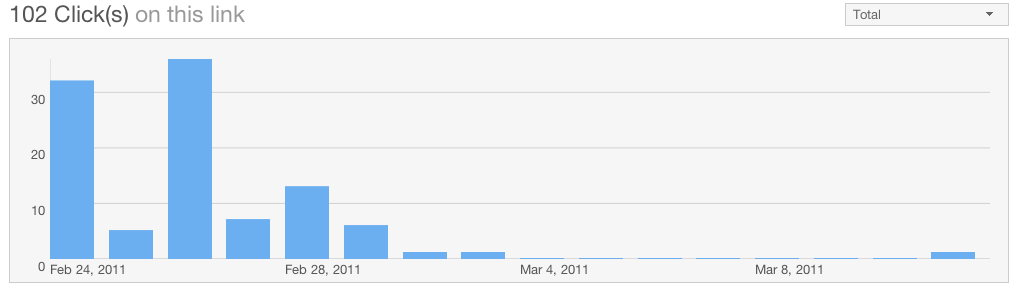
\includegraphics[width=0.7\linewidth]{bitly.png}}
    \subfigure[1,009 absolute pageviews of the extension as of Analytics.]{\label{fig:edge-b}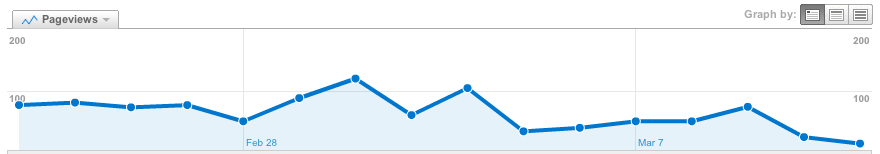
\includegraphics[width=0.7\linewidth]{all-traffic.png}}
    \subfigure[Distribution of named entity occurrences as of Analytics.]{\label{fig:edge-c}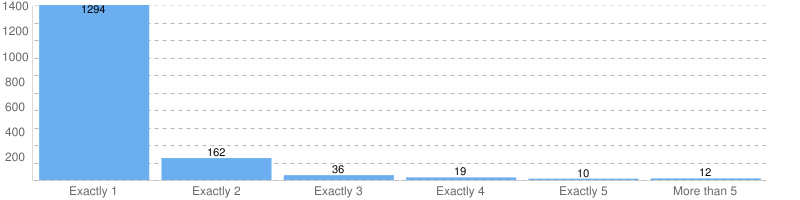
\includegraphics[width=0.7\linewidth]{distribution.png}}
  \end{center}
  \caption{Raw statistics.}
  \label{fig:traffic}
\end{figure}

\subsection{Top Read-about Named Entities}
In this section we present some statistics on the top read-about named entities (consumers' view), which, again, does not necessarily correspond to the most tweeted-about named entities (producers' view, see Section~\ref{sec:twopular}). It is to be noted that our findings are at this point \textit{not} statistically significant due to a too small number of seven-day active users of our extension (also see Section~\ref{sec:criticism}), however, nevertheless reveal interesting trends when the results are interpreted with a grain of salt. Table~\ref{table:top10} shows the top 10 read-about named entities from February 24 to March 11. Looking at the data, we can see that the topic around the events in ``Libya" (rank 1 and 6) and its dictator ``Gaddafi"\footnote{See \url{http://en.wikipedia.org/wiki/2011_Libyan_uprising} for a summary of the events.} (rank 10) were of high interest to the tweet readers. Rank 7 is taken by the named entity ``iPad", which makes sense given the introduction of the iPad 2 on March 2, 2011\footnote{See \url{http://en.wikipedia.org/wiki/Ipad_2#History} for the details.}. Other named entities are not necessarily easily mappable to concrete events, however, the data suggests that ``Twitter" (rank 2), ``Google" (rank 3), and ``YouTube" (rank 5) are companies that tweet readers show a general interest in, which seems reasonable. For the named entity ``Linked Data" (rank 8), this is probably due to the social Twitter environment of the authors, but given the too small installation base is not representative. The named entity ``glossary of graph theory" (rank 9) is definitely an incorrectly extracted named entity, as the underlying term was always ``successor". We have no explanation for the popularity of ``United States dollar" (rank 4), however, suppose that it is a correctly recognized, albeit relatively meaningless because out of context, named entity, as the underlying term was in all cases ``USD".

\begin{table}[htb!]
\begin{center}
\begin{tabular}{lll}
\hline
Rank & Named Entity & Total Occurrences \\ 
\hline
1 & \url{http://dbpedia.org/resource/Libya} & 23 \\
2 & \url{http://dbpedia.org/resource/Twitter} & 21 \\
3 & \url{http://dbpedia.org/resource/Google} & 13 \\
4 & \url{http://dbpedia.org/resource/United_States_dollar} & 10 \\
5 & \url{http://dbpedia.org/resource/YouTube} & 10 \\
6 & \url{http://rdf.freebase.com/ns/en/libya} & 10 \\
7 & \url{http://dbpedia.org/resource/IPad} & 9 \\
8 & \url{http://rdf.freebase.com/ns/en/linked_data} & 9 \\
9 & \url{http://dbpedia.org/resource/Glossary_of_graph_theory} & 8 \\
10 & \url{http://dbpedia.org/resource/Muammar_al-Gaddafi} & 8 \\
\hline \\
\end{tabular}
\end{center}
\caption{Top 10 read-about named entities (for rank 4, the original URL was \texttt{http://d.opencalais.com/genericHasher-1/736a403d-157b-3e80-86a7-acc404607cb2})}\label{table:top10}
\end{table}

\subsection{Tracking Of Named Entities Over Time}
Using Google Analytics, named entities (i.e., events in the sense of Google Analytics, as outlined in Section~\ref{sec:techimp}) can be easily tracked over time. As an example, Figure~\ref{fig:overtime-edge-a} shows  the occurrences over time for the named entity ``iPad". Albeit the numbers are not statistically significant, the peak of interest is on March 2, the day where the iPad 2 was revealed, and the second highest peak is on March 1, the day before the announcement, where media was atwitter with expectation of the device. Another example is given in Figure~\ref{fig:overtime-edge-b}, which shows the occurrences of the named entity ``tsunami". Japan was hit by an earthquake followed by a tsunami on March 11, exactly where the peak is on the graph. Hence, the occurrence graphs indeed correspond to what we would expect.

\begin{figure}[ht!]
  \begin{center}
    \subfigure[Popularity of the named entity ``iPad" (actually ``iPad 2") over time (February 24 - March 11). The device was revealed on March 2, 2011.]{\label{fig:overtime-edge-a}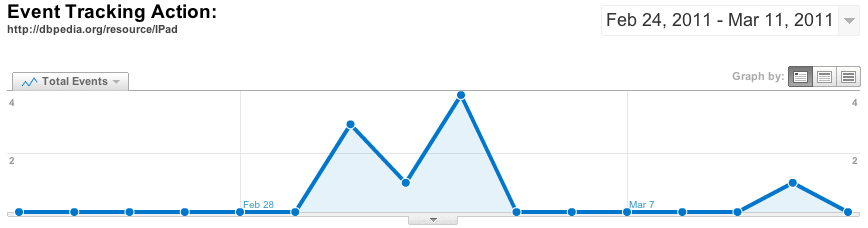
\includegraphics[width=0.495\linewidth]{ipad.png}}
    \subfigure[Popularity of the named entity ``tsunami" over time (March 10 - March 14). Japan was hit by an earthquake followed by a tsunami on March 11.]{\label{fig:overtime-edge-b}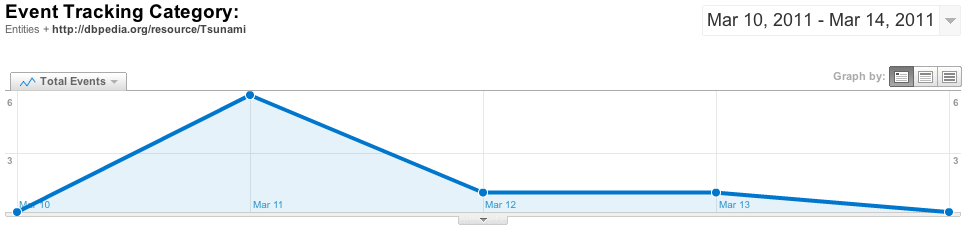
\includegraphics[width=0.495\linewidth]{tsunami.png}}
  \end{center}
  \caption{Popularity of named entities over time.}
  \label{fig:overtime}
\end{figure}

\subsection{Top Read-about Named Entities Pivoted By Country}
Japan was hit by an earthquake followed by a tsunami on March 11. As one would expect, this was reflected in the most read-about named entities for the period March 11 to March 14. The top 3 most read-about named entities for this period of time were ``tsunami" (8 occurrences), ``Japan" (7 occurrences), and ``earthquake" (4 occurrences). Table~\ref{table:pivotbycountry} shows the occurrences distribution pivoted by country. Again, our data set is too small to be statistically significant, however, the potential for this data to reveal new insights is promising. Given enough data, we could, e.g., provide an answer to the question whether among Twitter users the tsunami caused more interest in the American, or the European continent. As we use URIs as named entity identifiers, there is no ambiguity, and no language barriers (the English word ``earthquake" and the Spanish ``terremoto" will both be represented by, e.g., \url{http://dbpedia.org/resource/Earthquake}).

\begin{table}[htb!]
\begin{center}
\begin{tabular}{lllllllll}
\hline
Entity & Total & Germany & Finland & United States & Chile & India & Netherlands & Italy \\
\hline
\url{dbp:Tsunami} & 8 & 3 & 2 & 1 & 1 & 0 & 1 & 0 \\
\url{dbp:Japan} & 7 & 2 & 3 & 1 & 0 & 0 & 0 & 1 \\
\url{dbp:Earthquake} & 4 & 2 & 1 & 0 & 0 & 1 & 0 & 0 \\
\hline \\
\end{tabular}
\end{center}
\caption{Top 3 most read-about named entities (March 10 - March 14) pivoted by country, sorted by `Total". The prefix \texttt{dbp} stands for \texttt{http://dbpedia.org/resource}.}\label{table:pivotbycountry}
\end{table}

\subsection{Criticism Of the Approach}\label{sec:criticism}
The quality of the extracted named entities from tweets rises and falls with the quality of the Natural Language Processing step. Not being in the domain of NLP ourselves, we try to address the uncertain quality by using several NLP services in parallel. We found the approach to work well, with only few false results. As outlined in Section~\ref{sec:techimp}, we always track the source and entity name in the \texttt{label} field of the overloaded Analytics event, which allows us to go back from a named entity's representing URI to the originating terms, which oftentimes already permits to judge the quality of the named entity and its relevance.

We found the biggest issue to be to get a critical mass of Twitter users to install the extension in order to get more reliable data. We were very open in our extension description that data was tracked via Analytics, which might have caused privacy-aware users to stay away from it. Twitter itself uses Google Analytics (as per the Twitter.com source code with the account ID ``UA-30775-6"), however, states this fact only in a discreetly mentioned privacy policy\footnote{\url{http://twitter.com/privacy}} as required by the Google Analytics terms and conditions\footnote{\url{http://www.google.com/intl/en/analytics/tos.html}}. One could think of a similar approach for the extension.

Currently the user base also is still biased by the authors' social structure (more people have found the extension via Twitter than via the Chrome Web Store, which is the primary discovery channel for Chrome extensions). From a user's point of view, this is also due to the extension's primary purpose (display extracted named entities in tweets), which apart from users interested in the Semantic Web or NLP technologies is not an appealing reason for average Twitter users to install such extension. One could imagine bundling (hiding) the tweet analysis part of the extension with a more generic use case for a Twitter extension, like, e.g., a short URL unshortener, or a Twitter auto-refresher extension.

\section{Related Work}\label{sec:relatedwork}
As stated in Section~\ref{sec:introduction}, Twitter Trends is both an active field of academic and industry research, but also a playground for social media hobbyists. In the following we present four examples from these categories.

\subsection{Linked Open Social Signals (TWARQL)}
In the Linked Open Social Signals project~\cite{Mendes:LOSS} Mendes et al. investigate the representation of microposts as Linked Open Data (the authors call the opinions, observations, and suggestions contained in microposts ``social signals", hence the project name Linked Open Social Signals). Mendes et al. address the problem of information overload caused by the sheer amount of microposts. While the micropost community has come up with hashtags in order to categorize microposts, these hashtags are ambiguous and have to be explicitly added to the micropost by the author. Given the typical length limitations of microposts (often 140 characters), sometimes hashtags are left out in favor of more text. The project's main goal is thus to enable collective analysis of social signals for sense-making by using Linked Open Data principles in combination with realtime push models. The authors maintain a client-side JavaScript application\footnote{\url{http://knoesis1.wright.edu/twarql/query.html}} allowing for users to search for tweets matching a customizable SPARQL query or to subscribe to tweet streams in a realtime ``push" way, filtered according to the user's request (so-called concept feeds).

\subsection{Twitris 2.0}
With Twitris 2.0~\cite{Jadhav:Twitris}, Jadhav et al. present an application to find out what is being said about an event and when, to detect how topics of discussion are changing over a period of time, and finally to check whether there are regional differences in the opinions on a given topic. The approach consists of picking trending hashtags from Twitter, which are then expanded by data from Google Insights for Search\footnote{\url{http://www.google.com/insights/search/}}. Using this set of search terms, related hashtags are then searched on Twitter to detect topic drifts. In order to locate the origin of a tweet, Twitris uses the approximation of the location given in the user's Twitter profile. This approach works well if there is geocodable data (like ``Austin, Texas"), however, fails if there is generic data (like ``somewhere under the rainbow"). Tweets about a given set of topics can then be examined on a map view, enriched by relevant photo and video content. For each location hotspot a tag cloud with related tags is displayed, and the data can be sliced by time.

\subsection{Semantic-MicrOBlogging (SMOB)}
SMOB~\cite{Passant2008} by Passant et al. is a Semantic MicroBlogging framework that enables a distributed, open and semantic microblogging experience based on Semantic Web and Linked Data technologies. Microposts get annotated with common vocabularies like FOAF\footnote{\url{http://www.foaf-project.org/}} and SIOC\footnote{\url{http://sioc-project.org/}}. SMOB relies on distributed autonomous hubs that communicate with each other to exchange microblog posts and subscriptions, which can also be cross-posted to Twitter. The authors suggest the use of meaningful hashtags such as \texttt{\#dbp:Eiffel\_Tower}, or \texttt{\#geo:Paris\_France}, in the style of RDF prefixes for DBpedia and GeoNames. SMOB allows for manually annotating hashtags with URIs and RDF, with the objective of making microposts accessible for, e.g., lookup services such as Sindice\cite{Tummarello:Sindice}.

\subsection{Twopular}\label{sec:twopular}
Twopular\footnote{\url{http://twopular.com/}} is an experiment by Martin Dudek with the objective of analyzing current Twitter trends. Therefore, for a given set of at the particular moment current trends the most recents tweets are obtained, and in an interval of five minutes run through the OpenCalais Web service in order to find tags. By having tags for Twitter trends, another way of searching for trends -- and more importantly the possibility to interrelate trends based on tag similarity -- gets enabled.

\begin{comment}
\begin{figure}[ht!]
  \centering
  \includegraphics[width=0.85\linewidth]{twopular-trends.png}
  \caption{Screenshot of the Twopular trends page.}
  \label{fig:twopular}
\end{figure}
\end{comment}

\section{Future Work And Conclusion}\label{sec:conclusion}
In this paper, we have suggested a solution for obtaining a consumers' point of view on Twitter trends. Rather than measuring the ``trendiness" of terms/hashtags in tweets being produced, we measure the ``trendiness" of named entities in tweets being consumed using Google Analytics. This is not only interesting \textit{per se}, but together with the ``by-product" of classical Web analysis allows for even richer insights into, e.g., the location of users interested in a certain trend, sliceable back to any point (or period of time) in history where there is data available.

Future work can go in different directions. First, it is desirable to reach a broader user base through bundling the data analysis part of the extension with a more generic Twitter extension that solves a broader use case. Second, parts of the collected data could be fed back to the users (top \textit{n} read-about entities during the last \textit{x} hours in a \textit{region}). Third, the commercial potential of the collected data is promising, albeit regionally different privacy laws may apply that prevent use of such data. There are potential new social media analysis tools that could be based on tweet consumers' points of view on Twitter trends. We have barely scratched the surface of what is possible.
%%%%%%%%%%%%%%%%%%%%%%
%%%  Bibliography  %%%
%%%%%%%%%%%%%%%%%%%%%%

% The following two commands are all you need in the
% initial runs of your .tex file to
% produce the bibliography for the citations in your paper.
\bibliographystyle{abbrv}
\bibliography{typeinst}

\end{document}
